\documentclass[titlepage, 11pt]{article}
\usepackage[a4paper, total={6in, 9.5in}]{geometry}
\usepackage{graphicx}
\usepackage{amsmath,amsfonts,amssymb}
\usepackage{listings}
\usepackage{booktabs}
\usepackage[T1]{fontenc}
\usepackage{listings}
\usepackage{color}
\usepackage{minted}
\usepackage[colorlinks=true, linkcolor=blue, urlcolor=blue, citecolor=blue, pdfborder={0 0 255}]{hyperref}
\usepackage{colortbl}
\usepackage{url}
\usepackage{xcolor}
\usepackage{caption}
\usepackage{subcaption}
\usepackage{dirtytalk}
\usepackage[semicolon, round]{natbib}
\usepackage[ruled]{algorithm2e}
\captionsetup[table]{skip=10pt}
\renewcommand{\vec}[1]{\mathbf{#1}}
\SetKwComment{Comment}{$\triangleright$\ }{}
% \hypersetup{%
% 	colorlinks=true,
% 	linkcolor=blue,
% 	linkbordercolor={0 0 1}
% }

% \renewcommand\lstlistingname{Algorithm}
% \renewcommand\lstlistlistingname{Algorithms}
% \def\lstlistingautorefname{Alg.}

% \lstdefinestyle{Python}{
% 	language        = Python,
% 	frame           = lines, 
% 	basicstyle      = \footnotesize,
% 	keywordstyle    = \color{blue},
% 	stringstyle     = \color{green},
% 	commentstyle    = \color{red}\ttfamily
% }

% \setlength{\parindent}{0.0in}
% \setlength{\parskip}{0.05in}

\newcommand{\argmin}{\mathop{\mathrm{argmin}}}
\newcommand{\argmax}{\mathop{\mathrm{argmax}}}
\newcommand{\minimize}{\mathop{\mathrm{minimize}}}
\newcommand{\maximize}{\mathop{\mathrm{maximize}}}
\newcommand{\st}{\mathop{\mathrm{subject\,\,to}}}
\newcommand{\dist}{\mathop{\mathrm{dist}}}
\newcommand{\norm}[1]{\left\lVert#1\right\rVert}
\renewcommand{\vec}[1]{\mathbf{#1}}

\def\R{\mathbb{R}}
\def\E{\mathbb{E}}
\def\P{\mathbb{P}}
\def\S{\mathbb{S}}
\def\Cov{\mathrm{Cov}}
\def\Var{\mathrm{Var}}
\def\half{\frac{1}{2}}
\def\quat{\frac{1}{4}}
\def\sign{\mathrm{sign}}
\def\supp{\mathrm{supp}}
\def\th{\mathrm{th}}
\def\tr{\mathrm{tr}}
\def\dim{\mathrm{dim}}
\def\dom{\mathrm{dom}}

\title{
{EE1103: Numerical Methods} \\~\\
{\vlarge Programming Assignment {\#} 6}\\
}\author{ANIRUDH B S, EE21B019\\
Collaborators: & AMIZHTHNI P R K, EE21B015
 & ANKITA HARSHA MURTHY, EE21B020}
\date{\today}

\begin{document}
\maketitle

\setcounter{page}{0}
\tableofcontents
\listoffigures
\listoftables
\newpage

\section{Problem 1}
\noindent Consider the following differential equation
\begin{equation*}
    \frac{dy}{dt} = yt^{3} - 1.5y
\end{equation*} 
over the interval $t = 0$ to $2$. It is given that $y(0) = 1$. Solve the following parts:

\begin{itemize}
    \item [(a)] Write the analytical solution for the differential equation.
    
    \item [(b)] Numerically solve the same by applying the following methods. Use step size $h= 0.1$, $0.25$ and $0.5$.
    \begin{itemize}
        \item Euler's Method
        \item Heun's Predictor-Corrector Method
        \item Midpoint Method
        \item Fourth Order Runge Kutta Method
    \end{itemize}

\noindent For each value of $h$, plot the results from across ALL methods along with the true value, on the same graph. 

    \item [(c)] Report the run time for each method.
    
    \item [(d)] For each value of $h$, tabulate the absolute error of $y(2)$ for the different methods with respect to the true value. Infer the quality of the methods in terms of the error obtained.
    (Table should have $h$ in the rows and the error from different methods as column entries; you can choose to use more values of $h$ than estimated above, to prove your point)

\end{itemize}

\subsection{Approach}

In this problem, I shall exploit the following methods and compare their efficacy in solving linear ordinary differential equations. 
\begin{itemize}
    \item [(1)] Euler's Method 
    \item [(2)] Heun's Predictor Corrector Method
    \item [(3)] Mid-Point Method
    \item [(4)] 4th Order Runge Kutta Method
\end{itemize}

%%%%%%%%%%%%%%%%%%%%%%%%%%%%%%%%%%%%%%%%%%%%%%%%%%%%%%

\subsection{Algorithm}
In this section,I shall present the pseudocode/flowchart of the algorithm used to solve the problem.

The pseudocode for the problem is provided in Algorithm~\ref{alg1}, Algorithm~\ref{alg2}, Algorithm~\ref{alg3} and Algorithm~\ref{alg4}.
\begin{center}
\begin{algorithm}[H]\label{alg1}

\SetAlgoLined

INPUT h \\
n $\gets$ $\frac{2}{h}$ \\
$x_i$ $\gets$ 0\\
$y_i$ $\gets$ 1\\
\For{$i=1$ to n}{
 $y_{i+1}$ $\gets$ $y_i$ + $f(x_i,y_i)h$ \\
  $x_{i+1}$ $\gets$ $x_i + h$\\
 $x_{i}$ $\gets$ $x_{i+1}$ \\
 $y_{i}$ $\gets$ $y_{i+1}$ \\
 $y_{true}$ $\gets$  $e^{\frac{x_i^4-6x_i}{4}}$\\
 $e_a$ $\gets$ $|y_{i}-y_{true}|$ \\
}

 \caption{Euler's Method}
\end{algorithm}    
\end{center}

\begin{center}
\begin{algorithm}[H]\label{alg2}

\SetAlgoLined

INPUT h \\
n $\gets$ $\frac{2}{h}$ \\
$x_i$ $\gets$ 0\\
$y_i$ $\gets$ 1\\
\For{$i=1$ to n}{
 $y_{i+1}^{\circ}$ $\gets$ $y_i$ + $f(x_i,y_i)h$ \\
$y_{i+1}$ $\gets$ $y_i$ + $\frac{f(x_i,y_i)+f(x_{i+1},y_{i+1}^{\circ})}{2}h$ \\
 $x_{i+1}$ $\gets$ $x_i + h$\\
 $x_{i}$ $\gets$ $x_{i+1}$ \\
 $y_{i}$ $\gets$ $y_{i+1}$ \\
 $y_{true}$ $\gets$  $e^{\frac{x_i^4-6x_i}{4}}$\\
 $e_a$ $\gets$ $|y_{i}-y_{true}|$ \\
}

 \caption{Heun's Predictor-Corrector Method}
\end{algorithm}    
\end{center}

\begin{center}
\begin{algorithm}[H]\label{alg3}

\SetAlgoLined

INPUT h \\
n $\gets$ $\frac{2}{h}$ \\
$x_i$ $\gets$ 0\\
$y_i$ $\gets$ 1\\
\For{$i=1$ to n}{
 $y_{i+\frac{1}{2}}$ $\gets$ $y_i$ + $f(x_i,y_i)\frac{h}{2}$ \\
$y_{i+1}$ $\gets$ $y_i$ + $f(x_{i+\frac{1}{2}},y_{i+\frac{1}{2}})h$ \\
 $x_{i+1}$ $\gets$ $x_i + h$\\
 $x_{i}$ $\gets$ $x_{i+1}$ \\
 $y_{i}$ $\gets$ $y_{i+1}$ \\
 $y_{true}$ $\gets$  $e^{\frac{x_i^4-6x_i}{4}}$\\
 $e_a$ $\gets$ $|y_{i}-y_{true}|$ \\
}

 \caption{Mid-Point Method}
\end{algorithm}    
\end{center}

\begin{center}
\begin{algorithm}[H]\label{alg4}

\SetAlgoLined

INPUT h \\
n $\gets$ $\frac{2}{h}$ \\
$x_i$ $\gets$ 0\\
$y_i$ $\gets$ 1\\
\For{$i=1$ to n}{
 $k_1$ $\gets$ $f(x_i,y_i)$\\
$k_2$ $\gets$ $f(x_i+\frac{h}{2},y_i+\frac{k_1h}{2})$\\
$k_3$ $\gets$ $f(x_i+\frac{h}{2},y_i+\frac{k_2h}{2})$\\
$k_4$ $\gets$ $f(x_i+h,y_i+k_3h)$\\
$y_{i+1}$ $\gets$ $y_i$ + $(k_1+2k_2+2k_3+k_4)\frac{h}{6}$ \\
 $x_{i+1}$ $\gets$ $x_i + h$\\
 $x_{i}$ $\gets$ $x_{i+1}$ \\
 $y_{i}$ $\gets$ $y_{i+1}$ \\
 $y_{true}$ $\gets$  $e^{\frac{x_i^4-6x_i}{4}}$\\
 $e_a$ $\gets$ $|y_{i}-y_{true}|$ \\
}

 \caption{4th Order Runge-Kutta Method}
\end{algorithm}    
\end{center}
%%%%%%%%%%%%%%%%%%%%%%%%%%%%%%%%%%%%%%%%%%%%%%%%%%%%%%
\subsection{Results}

In this section, I shall plot the graphs/table that provide an overview of my findings.

We plot the graphs showing the error percentage as a function of the number of terms considered while approximating $f(n)$ In Figure~\ref{fig:q111a}, Figure~\ref{fig:q111b} and Figure~\ref{fig:q111c} . The results are also summarized in Table~\ref{tab:table2}.

\begin{itemize}
    \item [(a)] The analytical solution obtained is y(t) = $e^{\frac{t^4-6t}{4}}$. We obtain the same by variable separation method. Thus, the analytical solution is 
    \begin{equation}
        y(t) = e^{\frac{t^4-6t}{4}}
    \end{equation}
    \item [(b)] The results obtained for different methods for various h are given below in the Table ~\ref{tab:table2}
    \begin{table}[!htb]
    \caption{Value of y(2) obtained using various techniques}
    \centering
    \begin{tabular}{c|c|cccc}
    \toprule
    \textbf{$h$}& \textbf{True} & \textbf{Euler}& \textbf{Heun}  & \textbf{Mid-Point} & \textbf{Runge-kutta} \\
    \midrule
         0.10 & 2.718282 & 1.259499 &	2.610839	&2.507048 &	2.716550 \\
         0.25 & 2.718282 &	0.529695 &	2.320435 &	2.029023 &	2.682811 \\
         0.50 & 2.718282 &	0.113525 &	1.884185 &	1.591802 &	2.513072 \\
    \bottomrule
    \end{tabular}
    \label{tab:table2}
\end{table}
\begin{figure}[!tbh]
  	\centering
  	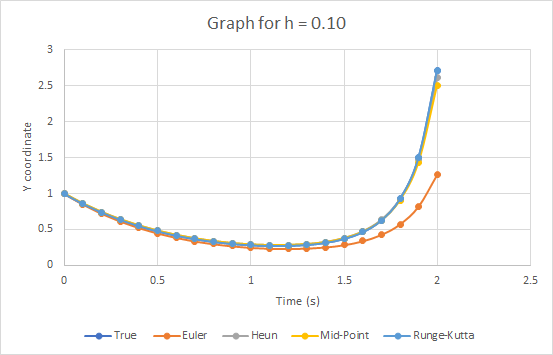
\includegraphics[width=0.9\textwidth]{G0.1.png} 
  	\caption{Graph obtained using various techniques for h = 0.10.}
  	\label{fig:q111a} 
\end{figure}
\begin{figure}[!tbh]
  	\centering
  	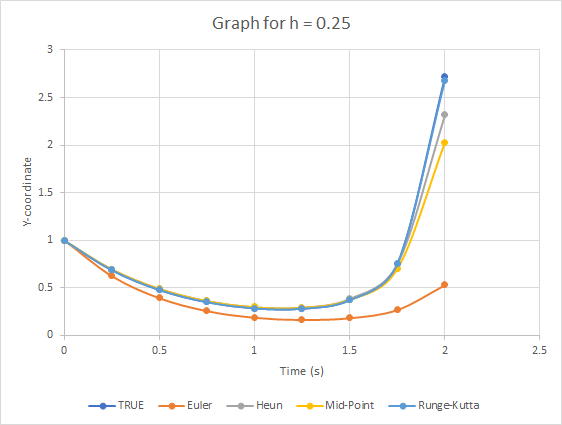
\includegraphics[width=0.9\textwidth]{G0.25.png} 
  	\caption{Graph obtained using various techniques for h = 0.25.}
  	\label{fig:q111b} 
\end{figure}
\begin{figure}[!tbh]
  	\centering
  	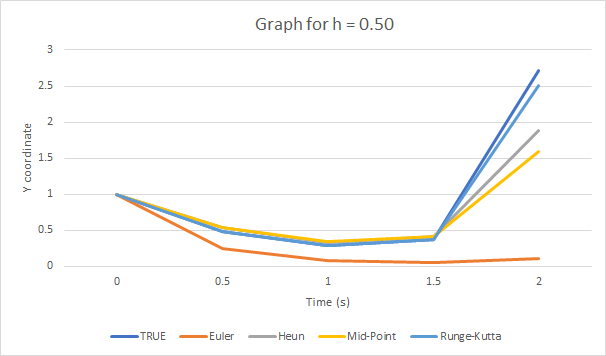
\includegraphics[width=0.9\textwidth]{G0.50.png} 
  	\caption{Graph obtained using various techniques for h = 0.50.}
  	\label{fig:q111c} 
\end{figure}
 \item [(c)] The run time for various methods for different values of h are tabulated in Table ~\ref{tab:mytable}. 
 \begin{table}[!tbh]
     \centering
     \begin{tabular}{c|cccc}
          \textbf{h} & \textbf{Euler} & \textbf{Heun} & \textbf{Mid-Point} & \textbf{Runge-Kutta}   \\
          \hline
          0.10 & 0.000167 & 0.000236 & 0.000189 & 0.000190 \\
          0.25 & 0.000128 & 0.000153 & 0.000170 & 0.000145 \\
          0.50 & 0.000101 & 0.000101 & 0.000064 & 0.000092 \\
     \end{tabular}
     \caption{Run Time for various methods }
     \label{tab:mytable}
 \end{table}
 \item [(d)]The errors obtained for different methods for various h are given below in the Table ~\ref{tab:table4}
 \begin{table}[!htb]
    \caption{Absolute Error in computation of y(2) using various techniques}
    \centering
    \begin{tabular}{c|cccc}
    \toprule
    \textbf{$h$}&  \textbf{Euler}& \textbf{Heun}  & \textbf{Mid-Point} & \textbf{Runge-kutta} \\
    \midrule
         0.10 & 1.458783 & 0.107444 & 0.211235 & 0.001732 \\
         0.25 & 2.188587 & 0.397847	& 0.689259 & 0.035471 \\
         0.50 & 2.604756 & 0.834097& 1.126480 &	0.205209 \\
    \bottomrule
    \end{tabular}
    \label{tab:table4}
\end{table}
\begin{figure}[!tbh]
  	\centering
  	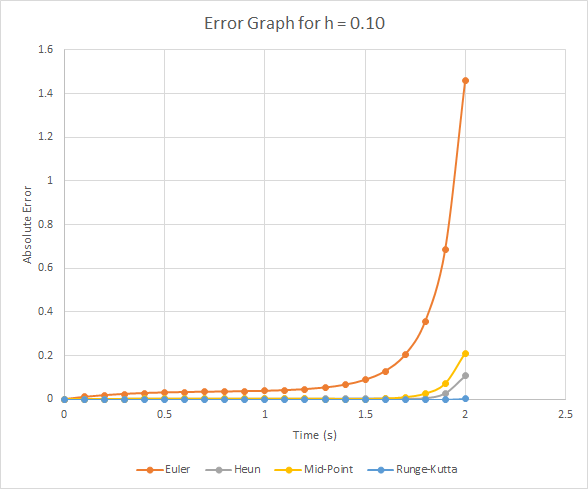
\includegraphics[width=0.9\textwidth]{EG0.1.png} 
  	\caption{Error Graph obtained using various techniques for h = 0.10.}
  	\label{fig:q112a} 
\end{figure}
\begin{figure}[!tbh]
  	\centering
  	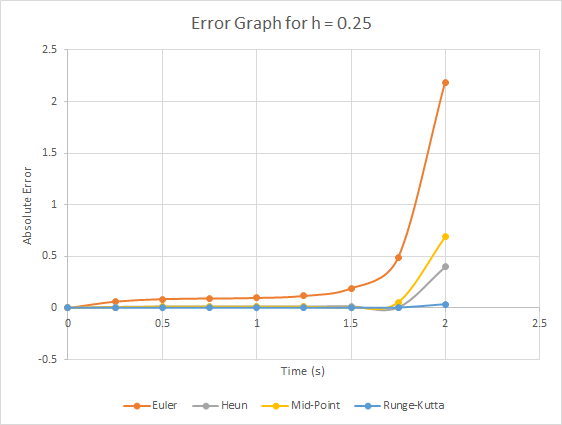
\includegraphics[width=0.9\textwidth]{EG0.25.png} 
  	\caption{Error Graph obtained using various techniques for h = 0.25.}
  	\label{fig:q112b} 
\end{figure}
\begin{figure}[!tbh]
  	\centering
  	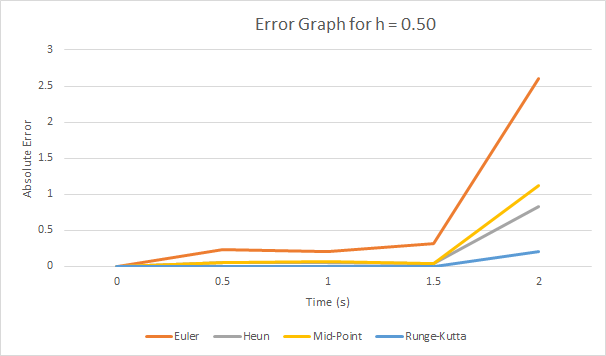
\includegraphics[width=0.9\textwidth]{EG0.50.png} 
  	\caption{Error Graph obtained using various techniques for h = 0.50.}
  	\label{fig:q112c} 
\end{figure}
\begin{figure}[!tbh]
  	\centering
  	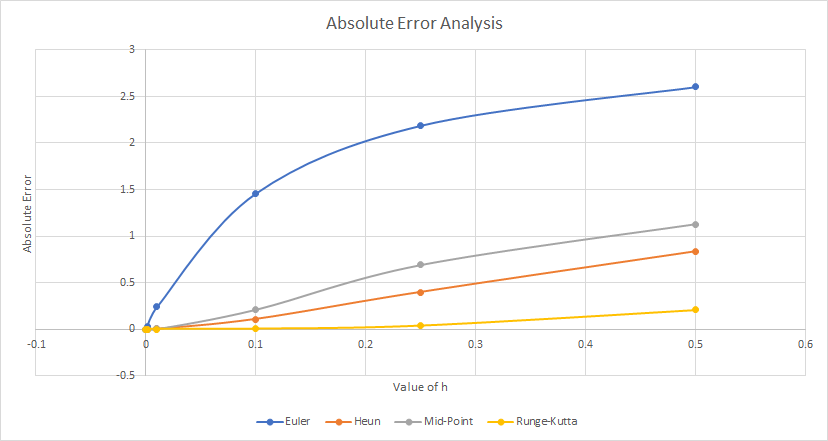
\includegraphics[width=0.9\textwidth]{Error_Graph.png} 
  	\caption{Error Graph for different value of h for different methods.}
  	\label{fig:q112d} 
\end{figure}
\end{itemize}


%%%%%%%%%%%%%%%%%%%%%%%%%%%%%%%%%%%%%%%%%%%%%%%%%%%%%%

\subsection{Inferences}
I deduce the following inferences from this problem :
\begin{itemize}
    \item [1] The efficiency of the four methods follow the below inequality with respect to the given problem.
    \begin{center}
        
        Euler's Method < Mid-Point Method < Heun's Method < 4th Order Runge-Kutta
    \end{center}
    \item [2] The Euler's Method as expected is inefficient. This is because, the Euler's Method offers a linear estimation of a differential equation, which is generally incorrect.
    \item [3] Another reasoning as to why the Euler's Method is inefficient could be that the Euler's Method considers only two terms of the Taylor Expansion of a function, while the 4th order Runge Kutta Method, as we shall see later, gives a better estimate by considering four terms. The error in Euler's Method is given by the following formula - (where $x_i$<c<$x_{i+1}$) 
    \begin{equation}
        E_t = \frac{f'(c)}{2}h^2
    \end{equation}
    \item [4] The Heun's Method provides a better estimate than the Euler's Method as it averages out the slope. The error in Heun's Method is given by the following formula - (where $x_i$<c<$x_{i+1}$)
    \begin{equation}
        E_t = \frac{f"(c)}{12}h^3
    \end{equation}
    \item [5] The mid point method uses the value of slope at the midpoint to extrapolate the function. As it may seem, the Mid-Point method does not work well in situations when the function grows or decays exponentially as is apparent in this problem.
    \item [6] The 4th Order Runge-Kutta Method considers 4 terms of the Taylor Series and thus provides a better approximation. The Runge-Kutta Method can be considered analogus to Simpson's Rule of Integration which generally provided accurate results.
    \item [7] The local and global truncation errors of various methods are listed in  Table ~\ref{tab:t1} - 
    \begin{table}[]
        \centering
        \begin{tabular}{c|c|c}
             \textbf{Method}& \textbf{Local Truncation Error} & \textbf{Global Truncation Error} \\
             \hline
             Euler's Method & O($h^2$)&O($h$) \\
             Heun's Method & O($h^3$)&O($h^2$)\\
             Mid-Point Method &O($h^3$) &O($h^2$)\\
             Runge-Kutta Method & O($h^5$) &O($h^4$)\\
        \end{tabular}
        \caption{Local and Global Truncation Errors}
        \label{tab:t1}
    \end{table}
    \item [8] For all the methods listed above, a general way to reduce error would be to decrease the step size. However, decreasing the step size would also increase the risk of time complexity and global truncation errors and global round off errors. The graph ~\ref{fig:q112d} and table ~\ref{tab:tab2} point out the same. It may not clearly be visible that error increases for lower h. This is because of limited accuracy of the computer. However, it is apparently seen in case of Runge-Kutta Method in the table.
    \begin{table}[]
        \centering
        \begin{tabular}{c|c|c|c|c}
            \textbf{h} & \textbf{Euler} & \textbf{Heun} &	\textbf{Mid-Point} &	\textbf{Runge-Kutta}\\
            \hline
0.00001	& 0.000255	&1.602x$10^{-9}$	&3.369x$10^{-9}$ &	4.50 x $10^{-11}$ \\
0.001&	0.025347 &	0.000016 &	0.000033 & 2.5x $10^{-11}$\\
0.01 &	0.237896 &	0.001502 &	0.003184 &	0.00000025 \\
0.1 &	1.458783 &	0.107444 &	0.211235 &	0.001732 \\
0.25 &	2.188587 &	0.397847 &	0.689259 &	0.035471 \\
0.5	& 2.604756	&0.834097 &	1.12648 &	0.205209 \\

        \end{tabular}
        \caption{Error vs h for different methods.}
        \label{tab:tab2}
    \end{table}
    \item [9] For h =0.10, we can see that the errors are lesser in comparision to the other values of h. As h increases, the error increases as it should be. In case of linear graphs, the Euler method best approximates the graph due to linear approximation.
    \item [10] As seen, the Runge- Kutta method is best suited for the given problem and the Euler method is ill-suited. 
\end{itemize}

%%%%%%%%%%%%%%%%%%%%%%%%%%%%%%%%%%%%%%%%%%%%%%%%%%%%%%

\subsection{Code}
The code used for the problem is mentioned in Listing~\ref{listing:1}, Listing~\ref{listing:2}, Listing~\ref{listing:3} and Listing~\ref{listing:4}. 

\inputminted[breaklines,
 mathescape,
 linenos,
 numbersep=5pt,
 frame=single,
 numbersep=5pt,
 xleftmargin=0pt]{c}{Euler.c}
 \captionof{listing}{Euler's Method}
\label{listing:1}

\inputminted[breaklines,
 mathescape,
 linenos,
 numbersep=5pt,
 frame=single,
 numbersep=5pt,
 xleftmargin=0pt]{c}{Heun.c}
 \captionof{listing}{Heun's Predictor Corrector Method}
\label{listing:2}

\inputminted[breaklines,
 mathescape,
 linenos,
 numbersep=5pt,
 frame=single,
 numbersep=5pt,
 xleftmargin=0pt]{c}{Midpoint.c}
 \captionof{listing}{Mid-Point Method}
\label{listing:3}

\inputminted[breaklines,
 mathescape,
 linenos,
 numbersep=5pt,
 frame=single,
 numbersep=5pt,
 xleftmargin=0pt]{c}{Rungekutta.c}
 \captionof{listing}{Runge Kutta Method}
\label{listing:4}


%%%%%%%%%%%%%%%%%%%%%%%%%%%%%%%%%%%%%%%%%%%%%%%%%%%%%%

\subsection{Contributions}
In the above problem, \textit{my original contributions} are - 
\begin{itemize}
    \item Designing of the Algorithm and Code
    \item Tabulation of Results
    \item Plotting the graphs on MS Excel
    \item Drawing conclusions by looking at the Results obtained.
    \item Writing the report in LaTeX. 
\end{itemize}

%%%%%%%%%%%%%%%%%%%%%%%%%%%%%%%%%%%%%%%%%%%%%%%%%%%%%%

\subsection{Alternate Methods}
\begin{itemize}
    \item [1] The Euler's Method is clearly incompetent. It could be replaced by a second-order Runge-Kutta method like a Heun's Method or a Ralston's Method.
    \item [2] The Mid-Point Method is the analog to the Md-Point Method of Integration, similarly, the Heun's Method and 4th order Runge Kutta methods correspond to Trapezoid and Simpson's Rule. 
    \item [3] Instead of the Mid-Point Method, we could exploit the Third-Order Runge Kutta methods. 
    \item [4] In applications requiring higher efficiency, we could take up Higher Order Runge Kutta methods. For most practical purposes, the Fourth-Order Runge Kutta method serves the purpose.
    \item [5] There are several other Runge-Kutta methods which could be used depending upon the situation and the degree of accuracy. Here are some of the \href{https://en.wikipedia.org/wiki/List_of_Runge%E2%80%93Kutta_methods#Ralston's_method}{Runge-Kutta Methods}
\end{itemize}

\newpage
%%%%%%%%%%%%% END OF QUESTION 1 %%%%%%%%%%%%%%%%%%%%
\section{Problem 2}
\noindent Solve 
\begin{equation*}
    \frac{dy}{dt} = -100,000y + 99,999e^{-t}
\end{equation*}
over the interval from $t = 0$ to $2$ using the following methods. Note that $y(0) = 0$.

\begin{itemize}
    \item [(a)] Explicit Euler method, after estimating the step size required to maintain stability. 
    
    \item [(b)] Implicit Euler method with a step size of $0.1$.

\end{itemize}

\subsection{Approach}

In this problem, I will contrast between Explicit Euler Method considering stability and Implicit Euler Method. I shall also list the pros and cons of each method.
%%%%%%%%%%%%%%%%%%%%%%%%%%%%%%%%%%%%%%%%%%%%%%%%%%%%%%

\subsection{Algorithm}
In this section,I shall present the pseudocode/flowchart of the algorithm used to solve the problem.

The pseudocode for the problem is provided in Algorithm~\ref{alg5} and Algorithm~\ref{alg6}.
\begin{center}
\begin{algorithm}[H]\label{alg5}

\SetAlgoLined

GET h \\
n $\gets$ $\frac{2}{h}$ \\
$x_i$ $\gets$ 0\\
$y_i$ $\gets$ 0\\
\For{$i=1$ to n}{
 $y_{i+1}$ $\gets$ $y_i$ + $f(x_i,y_i)h$ \\
  $x_{i+1}$ $\gets$ $x_i + h$\\
 $x_{i}$ $\gets$ $x_{i+1}$ \\
 $y_{i}$ $\gets$ $y_{i+1}$ \\
 $y_{true}$ $\gets$  $e^{-x_i}-e^{-100000x_i}$\\
}

 \caption{Explicit Euler's Method}
\end{algorithm}    
\end{center}

\begin{center}
\begin{algorithm}[H]\label{alg6}

\SetAlgoLined

h $\gets$ 0.1 \\
n $\gets$ $\frac{2}{h}$ \\
$x_i$ $\gets$ 0\\
$y_i$ $\gets$ 0\\
$a$ $\gets$ 100000 \\
\For{$i=1$ to n}{
 $y_{i+1}$ $\gets$ $\frac{y_i+99999e^{-{x+h}}h}{1+ah}$ \\
  $x_{i+1}$ $\gets$ $x_i + h$\\
 $x_{i}$ $\gets$ $x_{i+1}$ \\
 $y_{i}$ $\gets$ $y_{i+1}$ \\
 $y_{true}$ $\gets$  $e^{-x_i}-e^{-100000x_i}$\\
}

 \caption{Implicit Euler's Method}
\end{algorithm}    
\end{center}
%%%%%%%%%%%%%%%%%%%%%%%%%%%%%%%%%%%%%%%%%%%%%%%%%%%%%%
\subsection{Results}


In this section, I shall plot the table that provide an overview of my findings.\\
The analytical solution of the question is y(x) = $e^{-x}-e^{-100000x}$

\begin{itemize}
    \item [(a)] Using Explicit Euler Method, we obtain y(2) as 0.135335. Here we have taken h = $10^{-6}$ and number of iterations to be n = 2 x $10^{6}$
    \item [(b)] Using Implicit Euler Method, we obtain y(2) as 0.135335. Here we have taken h = 0.1 and number of iterations to be 20. 
    \item [(c)] The Table ~\ref{tab:tabee} shows the values obtained using Explicit Euler Method. The Table ~\ref{tab:tabie} shows the values obtained using Implicit Euler Method.
    \item [(d)] From the Table ~\ref{tab:tabie}, it is clearly evident that the Implicit Euler Method at y(2) is 0.135335 which matches with the true value of 0.135335. 
    
    \begin{table}[!htb]
    \caption{Explicit Euler Method}
    \centering
    \begin{tabular}{c|c|c}
    \toprule
    \textbf{$t$}& \textbf{$y_{true}$}& \textbf{$y_{Explicit}$}   \\
    \midrule
         0.000000 & 0.000000 & 0.000000 \\
         0.000001 & 0.095162 & 0.099999\\
         0.000002 & 0.181267 & 0.189998\\
         0.000003 & 0.259179 & 0.270997 \\
         0.000004 & 0.329676 & 0.343896 \\
         0.000005 & 0.393464 & 0.409505\\
         0.000006 & 0.451182 & 0.468553 \\
         0.000007 & 0.503408 & 0.521696 \\
         0.000008 & 0.550663 & 0.569525 \\
         0.000009 & 0.593421 & 0.612570 \\
         0.000010 & 0.632111 & 0.651312 \\
         0.000050 & 0.993212 & 0.994796 \\
         0.000100 & 0.999855 & 0.999873 \\ 
         0.000200 & 0.999800 & 0.999800 \\
         1.999995 & 0.135336 & 0.135336 \\
         1.999996 & 0.135336 & 0.135336 \\
         1.999997 & 0.135336 & 0.135336 \\
         1.999998 & 0.135336 & 0.135336 \\
         1.999999 & 0.135335 & 0.135335 \\
         2.000000 & 0.135335 & 0.135335 \\
    \bottomrule
    \end{tabular}
    \label{tab:tabee}
\end{table}
 \begin{table}[!htb]
    \caption{Implicit Euler Method}
    \centering
    \begin{tabular}{c|c|c}
    \toprule
    \textbf{$t$}& \textbf{$y_{True}$}& \textbf{$y_{Implicit}$}   \\
    \midrule
0.000000 &	0.000000 &	0.000000 \\
0.100000 &	0.904837 &	0.904738 \\
0.200000 &	0.818731 &	0.818731 \\
0.300000 &	0.740818 &	0.740819 \\
0.400000 &	0.670320 &	0.670320 \\
0.500000 &	0.606531 &	0.606531  \\
0.600000 &	0.548812 &	0.548812 \\
0.700000 &	0.496585 &	0.496586 \\
0.800000 &	0.449329 &	0.449329 \\
0.900000 &	0.406570 &	0.406570 \\
1.000000 &	0.367879 &	0.367880 \\
1.100000 &	0.332871 &	0.332871 \\
1.200000 &	0.301194 &	0.301194 \\
1.300000 &	0.272532 &	0.272532 \\
1.400000 &	0.246597 &	0.246597 \\
1.500000 &	0.223130 &	0.223130 \\
1.600000 &	0.201897 &	0.201897 \\
1.700000 &	0.182684 &	0.182684 \\
1.800000 &	0.165299 &	0.165299 \\
1.900000 &	0.149569 &	0.149569 \\
2.000000 &	0.135335 & 0.135335 \\
    \bottomrule
    \end{tabular}
    \label{tab:tabie}
\end{table}
\end{itemize}

%%%%%%%%%%%%%%%%%%%%%%%%%%%%%%%%%%%%%%%%%%%%%%%%%%%%%%

\subsection{Inferences}
I deduce the following inferences from the problem :

\begin{itemize}
    \item [1] Choosing the right h is most important for getting the right solution in case of Explicit Euler Method. A value of h > 0.00002 leads to divergence of the solution to $\infty$ or -$\infty$ and is thus meaningless. Thus, a choice of h < 0.00002 is vital. 
    \item [2] As seen for a value of h = $10^{-6}$, the solution of the differential converges to the exact solution. Although the time complexity is higher for the same, yet the solution is a great approximation. 
    \item [3] For instance, a value of h = 0.1, leads to the solution going towards $\infty$ in approximately 20 iterations. Thus, the rate of divergence in this case is quite rapid.
    \item [4] In case of the implicit Euler Method, it converges for all h. This is true only for a exponentially decaying function. 
    \item [5] It is quite surprising to see that the Implicit Euler Method converges to the actual solution 0.135335 in exactly 20 iterations. Thus, it converges very rapidly. 
    \item [6] The rapid convergence of the Implicit Euler Method can be attributed to the geometric sequence thus generated. 
    \item [7] Since the Implicit Euler Method converges regardless of the step-size h, it is quite often termed as \textbf{Unconditionally stable.}
    \item [8] The choice of right step size becomes very critical in analysing systems that show rapid changes with respect to the independent variable.
    \item [9] The Implicit Euler Method is only first order accurate and can also be extended to second order or third order as the need be. 
    \item [10] In summary, the implicit Euler Method performs better than the Explicit Euler Method in terms of Time Complexity as well as Space complexity. However, it is not the best method as described before. Suitable  modifications could be done to increase the efficiency of either of the methods.
\end{itemize}

%%%%%%%%%%%%%%%%%%%%%%%%%%%%%%%%%%%%%%%%%%%%%%%%%%%%%%

\subsection{Code}
The code used for the problem is mentioned in Listing~\ref{listing:5} and Listing~\ref{listing:6}. 


\inputminted[breaklines,
 mathescape,
 linenos,
 numbersep=5pt,
 frame=single,
 numbersep=5pt,
 xleftmargin=0pt]{c}{Explicit_Euler.c}
 \captionof{listing}{Expicit Euler's Method}
\label{listing:5}

\inputminted[breaklines,
 mathescape,
 linenos,
 numbersep=5pt,
 frame=single,
 numbersep=5pt,
 xleftmargin=0pt]{c}{Implicit_Euler.c}
 \captionof{listing}{Implicit Euler's Method}
\label{listing:6}

%%%%%%%%%%%%%%%%%%%%%%%%%%%%%%%%%%%%%%%%%%%%%%%%%%%%%%

\subsection{Contributions}
In the above problem, \textit{my original contributions} are - 
\begin{itemize}
    \item Designing of the Algorithm and Code
    \item Tabulation of Results
    \item Plotting the graphs on MS Excel
    \item Drawing conclusions by looking at the Results obtained.
    \item Writing the report in LaTeX. 
\end{itemize}

%%%%%%%%%%%%%%%%%%%%%%%%%%%%%%%%%%%%%%%%%%%%%%%%%%%%%%

\subsection{Alternate Methods}

\begin{itemize}
    \item [1] The space and time complexity of the Explicit Euler Method is far greater than the Implicit Euler Method. Thus, the Implicit Euler Method can replace the Explicit Euler methods in applications requiring a short run time and higher accuracy. 
    \item [2] Just like we constrained the Euler method to h < 0.00002, we could find constraints for stability on Heun'S Method, Mid Point Method and other Runge Kutta Methods. This would increase the efficiency of the latter methods. 
    \item [3] There are several Multi-step Methods which could lead to a better efficiency. As the need be, we could use any of the Multi-Step Methods in our application. 
    \item [4] \href{https://encyclopediaofmath.org/wiki/Milne_method#:~:text=A%20finite%2Ddifference%20method%20for,y(a)%3Db.}{Milne's Method} can be used as an efficient alternative to the above problem.
    \item [5] \href{https://web.mit.edu/10.001/Web/Course_Notes/Differential_Equations_Notes/node6.html}{Adam's Method} can be used as an efficient alternative to the above problem.
\end{itemize}

\end{document}
